\documentclass{homework}
\usepackage{lipsum}
\usepackage{cancel}
\usepackage{amsthm}
\usepackage{cleveref}
\usepackage{upgreek}
\usepackage{mathrsfs}
\usepackage{tikz}
\usepackage{units}
\newtheorem{lemma}{Lemma}

\title{Kevin Joyce}
\course{Stat 542 - Applied Linear Models}
\author{Kevin Joyce}
\docdate{\today}
\begin{document} 
\newcommand{\figref}[1]{\figurename~\ref{#1}}
\renewcommand{\bar}{\overline}
\renewcommand{\hat}{\widehat}
\renewcommand{\SS}{\mathcal S}
\newcommand{\HH}{\mathscr H}
\newcommand{\mom}{\widetilde}
\newcommand{\mle}{\widehat \Uptheta}
\newcommand{\eps}{\varepsilon}
\newcommand{\todist}{\stackrel{D}\longrightarrow}
\newcommand{\toprob}{\stackrel{p}\longrightarrow}
\newcommand{\TTheta}{\overline{\underline \Theta} }
\newcommand{\del}{\partial}
\newcommand{\approxsim}{\overset{\cdotp}{\underset{\cdotp}{\sim}}}
\begin{longproblem}
  The concentration of mercury in a lake has been monitered for a number of years.  Measurements taken on a weekly basis yielded an average of \unit[1.20]{$\mathrm{mg/m^3}$} (milligrams per cubic meter) with a standard deviation of \unit[0.32]{mg/m\textsuperscript{3}}.  Following an accident at a smelter on the shore of the lake, 15 measurements produced the following mercury concentrations, as found in the data file {\bf \tt mercury.txt}:  
\begin{center}
\begin{verbatim}
1.60 1.45 1.77 1.59 1.61 1.43 1.08 2.07 1.07 1.16 1.79 0.85 1.34 2.11 1.07
\end{verbatim}
\end{center}

\subproblem{Construct a 95\% confidence interval for the mean mercury concentration after the accident.  Interpret your interval clearly \emph{in context of the problem.} }

\begin{solution}
  Denote each data as $y_i$.  Since the data is subject to measurement error,
  and a normal quantile plot reveals no striking indicators of non-normality,
  we assume that the sample mean is well-approximated by a normal distribution
  via the Central Limit Theorem (CLT).  Hence, the statistic $T = (\bar y -
  \mu)/(s/\sqrt n)$ is approximately distributed $t(n-1)$. So, the confidence interval
  is given by $\bar y_. \pm t_{n-1}(1-\alpha/2)\cdot s/\sqrt n$, which in this case is \unit[$\big(1.257,\,1.675\big)$]{mg/m\textsuperscript3}.
  That is, we are 95\% confident that the new true mean mercury concentration is between \unit[1.256]{mg/m\textsuperscript3} and \unit[1.675]{mg/m\textsuperscript3}.  
\end{solution}

\subproblem{Is there sufficient evidence that the mean mercury concentration has increased since the accident?  In answering this question, provide hypotheses with the parameter clearly defined, the values of the test statistic and p-value, and a conclusion \emph{in context of the problem}.  Note that no significance level was given, so don't make one up!}

\begin{solution}
  We test the hypothesis $\HH_0: \mu = \unit[1.20]{mg/m\textsuperscript3}$
  versus $\HH_a: \mu > \unit[1.20]{mg/m\textsuperscript3}$. The p-value for the given data is $P[ \bar y \ge 1.466 | \mu =
  1.20 ] \approx P[ T \ge 2.737 ] \approx 0.008$.  Hence, there is convincing
  evidence that the mean mercury level has risen since the accident.
\end{solution}

\subproblem{Assuming that the standard deviation of the mercury concentrations
is \unit[0.32]{mg/m\textsuperscript{3}}, calculate the power of the test to
detect mercury concentrations of 1.28,1.32,1.36, and
\unit[1.40]{mg/m\textsuperscript3} and produce a relevant graph of the power as
a function of this detectable value.}

\begin{solution} 
  Let us assume a fixed Type I error rate of $\alpha = .05$ and that each
  sample standard deviation will given an unbiased estimate of \unit[0.32]{mg/m\textsuperscript3}. Let the new mean concentration be given as $\mu_a \in\{ 1.28,1.32,1.36, 1.40\}$.  Then, the power of the test is given by $1 - P\big[\bar
  y \le \widehat{SE}\cdot t_{15}(.05) + 1.20 | \mu = \mu_a \big] = 1 - P\big[T \le
  t_{.05} + (1.20 - \mu_a)/(0.32/\sqrt{15})\big] $.  The following table gives the
  power for the various mercury concentrations.
  \renewcommand{\arraystretch}{1.4}
  \begin{tabular}{c|c c c c}
  \hline
  $\mu_a$ & 1.28&1.32&1.36& 1.40 \\
  Power & 0.992 &  0.997 &  0.999 &  \unit[$>$]0.999 \\\hline
  \end{tabular}
\end{solution}

\end{longproblem}
\newpage

\problem{A biologist wishes to estimate the effect of an antibiotic on the
growth of a particular bacterium by examining the mean amount of bacteria
present per plate of culture when a fixed amount of antibiotic is applied.
Previous experimentation with the antibiotic on this type of bacteria indicates
that the standard deviation of the amount of bacteria present is approximately
\unit[13]{cm\textsuperscript2}.  Use this information to determine the number
of observations (cultures that must be developed and then tested) to estimate
the mean amount of bacteria present, using a \unit[99]{\%} percent confidence
interval with a margin of error of \unit[3]{cm\textsuperscript2}.
}

\begin{solution}
  Recall that the general form of a confidence interval for $\mu$ is: $\bar y
  \pm z(1-\alpha/2) \cdot \sigma/\sqrt n = \bar y \pm E$ when $\sigma$ is
  assumed known and the population is normal or the sample size is sufficiently
  large.  Under these assumptions, we equate the margin of error $E = 3 = z(1-\alpha/2) \cdot \sigma/\sqrt n$ and solve for $n$
  to obtain
  $$
    n \ge \left(\frac{z(.995) \cdot 13}{3} \right)^2 \approx 124.6.
  $$
  So a sample size of at least $125$ will guarantee the given margin of error and confidence under the given assumptions.  
\end{solution}

\begin{longproblem}
\begin{wraptable}{r}{3in}
\renewcommand{\arraystretch}{1.3}
\begin{tabular}{c c c}
\hline
\multicolumn{3}{c}{Plant Height (inches)} \\ \hline
Pair & Cross-Fertilized & Self-Fertilized\\\hline
 1& 23.5  & 17.375\\
 2& 12     &20.375\\
 3& 21    & 20\\
 4& 22    & 20\\
 5& 19.125& 18.375\\
 6& 21.5  & 18.625\\
 7& 22.125& 18.625\\
 8& 20.375& 15.25\\
 9& 18.25 & 16.5\\
10& 21.625& 18\\
11& 23.25 & 16.25\\
12& 21    & 18\\
13& 22.125& 12.75\\
14& 23    & 15.5\\
15& 12    & 18\\\hline
\end{tabular}
\end{wraptable}

  Charles Darwin carried out an experiment to study whether seedlings from
  cross-fertilized plants tend to be superior to those from self-fertilized
  plants.  He covered a number of plants with fine netting so that insects
  would be unable to fertilize them.  He fertilized a number of flowers on each
  plant with their own pollen and he fertilized an equal number of flowers on
  the same plant with pollen from a distant plant.  (He did not say how he
  diced which flowers received which treatments.)  The seeds from the flowers
  were allowed to ripen and were set in wet sand to germinate.  He placed two
  seedlings of the same age in a pot, one from a seed of a self-fertilized
  flower and one from a seed of a cross-fertilized flower.  The data in the
  table to the right (and in the text file \texttt{darwin.txt}) are the heights
  of the plants at certain points in time.  [The fertilization experiments were
  described by Darwin in an 1878 book; these data were found in D.F. Andrews
  and A.M. Herzberg, \emph{Data}, New York: Springer-Verlag, 1985, pp. 9-12].
\end{longproblem}

\newpage
\subproblem{Create a histogram of these \emph{differences} and describe the distribution of these differences \underline{in context of the problem}.}

{\bf Solution:}

\begin{wrapfigure}{l}{0.5\textwidth}
\vspace{-20pt}
\begin{center}
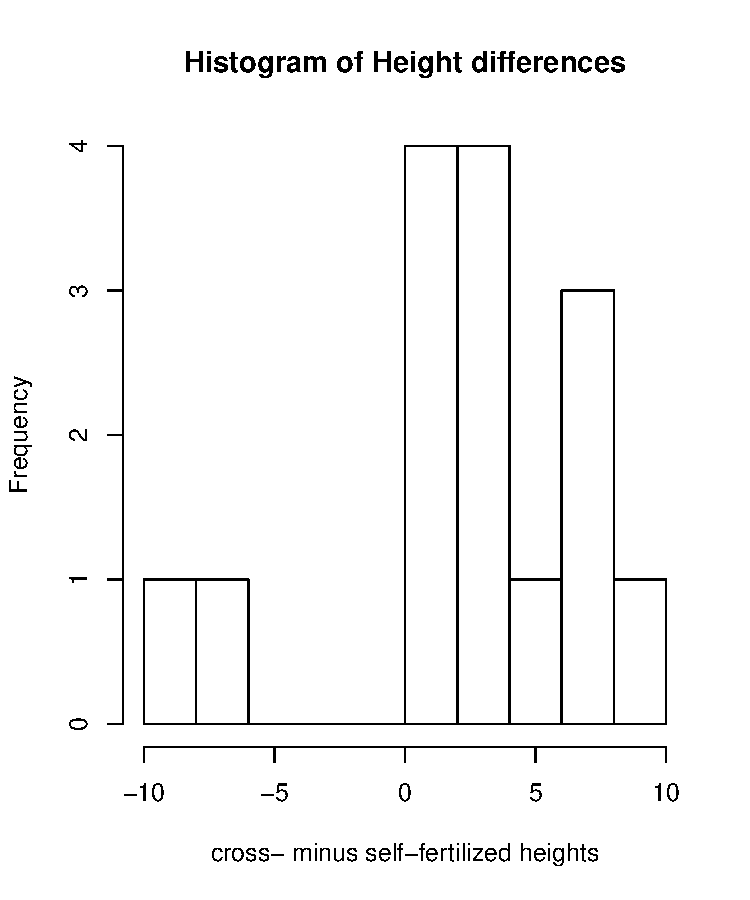
\includegraphics[width=.48\textwidth]{darwin_hist.pdf}
\end{center}
\vspace{-20pt}
\end{wrapfigure}
Generally, the data are centered slightly above 0 and vary from $-10$ to $10$.  There is a lack of data from -5 to 0, so the shape of the distribution could be argued to be bimodal with the right ``mode'' slightly right
skewed. There are only two points corresponding to the left ``mode'' and may be
outliers. It is difficult to discern since the sample size is relatively
small ($n=15$). In context of the problem, most of the cross-fertilized plants have
heights at least as large as the self-fertilized plants (other than two).  Of
those pairs where cross-fertilized plants are larger, most are with two to four
inches taller.  

\subproblem{ Test whether or not there was any difference in the mean plant
height for the two treatments using a paired t-test.  In doing so, give the
p-value for the test and a conclusion based on this p-value. [A paired t-test
can be performed in \texttt{R} using the \texttt{t.test} function with the
\texttt{paired=T} option.  This function will also produce a confidence
interval as required in the next part.]} 

\begin{solution} 
We test the hypotheses $\HH_0:$``The mean height of cross-fertilized plants is
equal to the mean height of self-fertilized plants,'' versus  $\HH_a:$``The mean
height of cross-fertilized plants is \emph{greater} than the self-fertilized plants.''
The $t$-based inference results in a $p$-value $<0.025$; hence, there is reasonably good evidence
that the mean cross-fertilized plant height is greater than that of the
self-fertilized plants.
\end{solution}

\subproblem{ Find a 95\% confidence interval for the mean difference in plant heights between the two treatments, and interpret this interval in the context of the problem. }

\begin{solution}
The confidence interval reported by \texttt{t.test}  is
$(0.471,\infty)$. Hence, we can conclude with 95\% confidence that the cross-fertilized height is at least \unit[0.471]{in.} greater than the self-fertilized height.  Although, I suspect that this interval corresponds to the rejection region associated with the test in (b), and is clearly not of the form $\widehat x_{\mathrm{diff}} \pm \widehat{SE}$. If we perform the $t$-test without the \texttt{alternative="greater"} option, the interval \unit[(0.004, 5.229)]{in.} was reported.
\end{solution}

\newpage

\subproblem{Is there any indication from the histogram in part (a) that the paired t-test may be inappropriate? Explain clearly.}

\begin{solution}
  This test is based on certain normality assumptions. Specifically, that each
  population (and hence their difference) are normal random variables.  The
  sample size is small such that large sample results (i.e. CLT) are not
  applicable.  The distribution of the difference could be interpreted as
  bell-shaped, but the lack of data from -5 to 0 is worrisome.  As remarked in
  part (a), the data could be interpreted as bimodal which is a non-normal
  characteristic.  Hence, either further assumption investigation or a non-parametric method may be appropriate.
\end{solution}

\begin{longproblem}
  Fuchs and Kenett (1987) presented data on citrus juice for fruits grown during a specific season at a specific location .  The sample size was 80 but many variables were measured on each sample.  Sample statistics for some of these variables are given below:
  \begin{center}
  \begin{tabular}{c c c c c c c c}
  Variable & BX & AC & SUG & K & FORM & PECT \\ \hline
  Mean & 10.4 & 1.3 & 7.7 & 1180.0 & 22.2 & 451.0 \\
  Variance & 0.38 & 0.036 & 0.260 & 43590.364 & 6.529 & 16553.996 \\\hline
  \end{tabular}
  \end{center}
  The variables are: BX - total soluble solids produced at \unit[20]{\textsuperscript oC}, AC - acidity as citric acid unhydrons, SUG - total sugars after inversion, K - potassium, FORM - formol number, PECT - total pectin.  Give a \unit[99]{\%} confidence interval for the population mean of each variable and give a \unit[99]{\%} prediction interval for each variable.  Test whether the mean of BX equals 10 units.  
\end{longproblem}

\begin{solution}
  Let us assume that each population satisfies conditions so that $t$-based inference is appropriate.  Then, in each case the confidence interval for the means is given by $\bar x_i \pm t_{79}(.995) \cdot s_i/ \sqrt{80}$ and the prediction intervals for the mean are given by $\bar x_i \pm t_{79}(.995) \cdot s_i \sqrt{ 1 + 1/80}$.  A summary of these intervals is given in the table below:
  \begin{center}
  \renewcommand{\arraystretch}{1.4}
  \begin{tabular}{c| l l}
  \hline
  Variable & 99\% Confidence Interval for Mean & 99\% Prediction interval\\ \hline
  BX & (10.218,10.582) & (8.763,12.037) \\
  AC & (1.244,1.356) & (0.796,1.804) \\
  SUG & (7.550,7.850) & (6.346,9.054) \\
  K & (1118.387,1241.613) & (625.483,1734.517) \\
  FORM & (21.446,22.954) & (15.414,28.986) \\
  PECT & (413.031,488.969) & (109.279,792.721) \\\hline
  \end{tabular}
  \end{center}

  We can test $\HH_0:$``The mean the mean total soluble solids produced at \unit[20]{\textsuperscript oC} equals 10'' versus $\HH_a:$``It doesn't equal 10'' using $t$-based inference which results in a $p$-value $< 10^{-7}$ indicating very strong evidence that the mean total soluble solids produced is not $10$.  We remark that such a result is not surprising due to the large ($n=80$) sample size.
\end{solution}

\begin{longproblem}
  Shewhart (1931,p. 62) reproduces Millikan's data on the charge of an electron, as given in the file \texttt{electron.txt}.  Check these data for outliers and nonnormality.  Make any adjustments to the data that are needed (data transformation, outlier removal, etc.) and explain these adjustments.  Compute a \unit[99]{\%} confidence interval for the population mean value.
\end{longproblem}

{\bf Solution:}

\begin{wrapfigure}{l}{.4\textwidth}
\vspace{-20pt}
\begin{center}
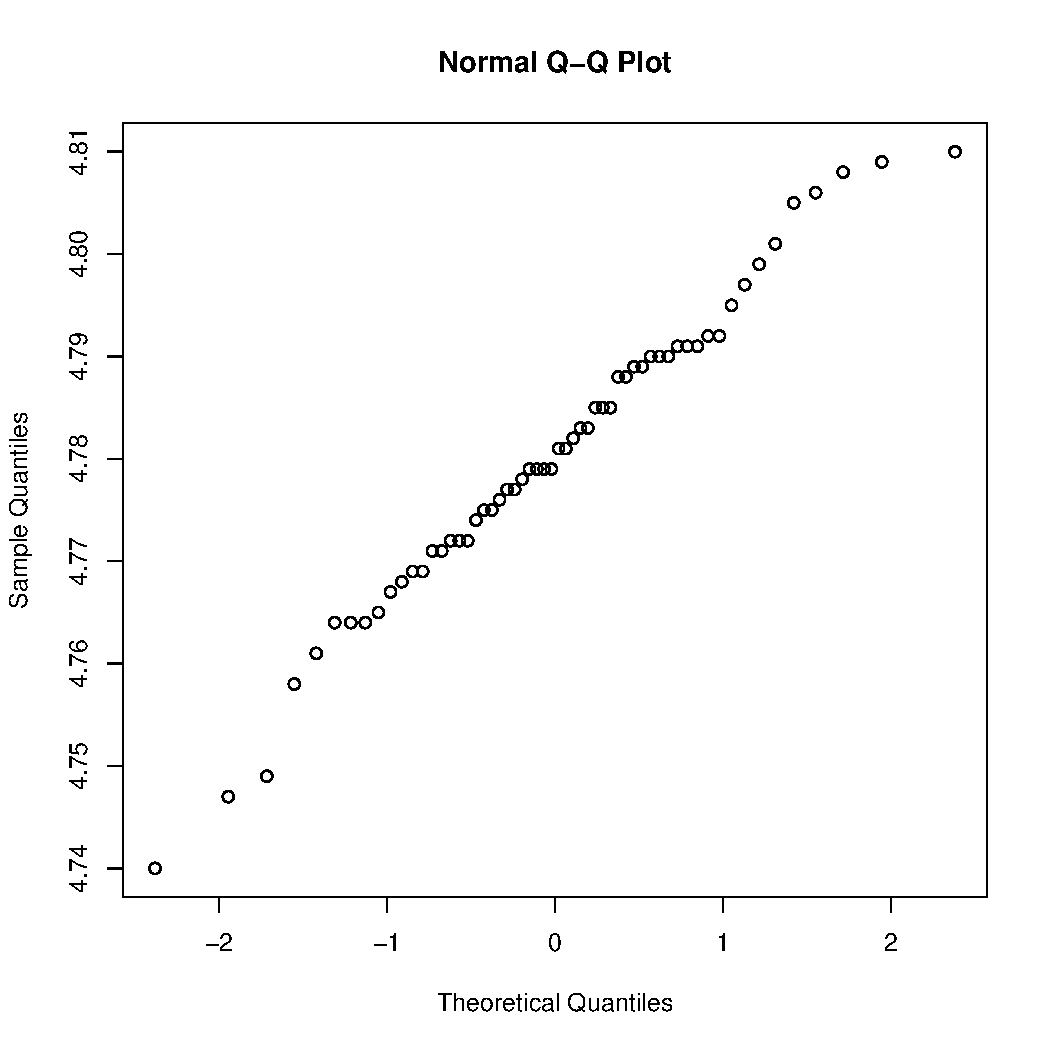
\includegraphics[width=.38\textwidth]{electron_normal.pdf}
\end{center}
\vspace{-20pt}
\end{wrapfigure}
  In the figure to the left, we plot the data against a sequence of estimates
  of the quantiles of the normal distribution; i.e. a qqplot.  The plot does
  not indicate much evidence for non-normality (the points seem to fit closely
  to a $45^\circ$ line). Formally, the Shapiro-Francia normality test does provide any
  statistical evidence for departures form normality.  Hence, we proceed
  with standard $t$-based inference without any transformation or outlier removal. The
  \unit[99]{\%} confidence interval for the mean charge is $\big(4.775, 4.786\big)$.

  \begin{longproblem}
  Problem 1, page 9 Faraway.  The dataset \texttt{teengamb}
  concerns a study of teenage gambling in Britain.  Make a numerical and
  graphical summapy of the data, commenting on any features that you find
  interesting.  Limit the output you present to a quantity that a busy reader
  woulde find sufficient to get a basic understanding of the data (about one
  page in length). [To access the data for this problem, you will first need to
  install and load the package \texttt{faraway} into \texttt R.  Once this is
  done, you can type \texttt{data(teengamb)} to read the teen gambling data
  into memory.  Typing \texttt{summary(teengamb)} will give you a summary of
  the variables in the data set and typing \texttt{help(teengamb)} will give
  you a detailed explanation of what each variable means, as well as the source
  reference for the data. 
  \end{longproblem}
  
  \begin{solution}
  Survey data on the gambling behavior of 47 British adolescents aged 13 to 14
  years old were collected in 1988 from a neighborhood comprehensive school in
  Exeter, Devon.  The pervasiveness of gambling among the population as well as
  how it can be described by other variables was of primary interest by the
  researchers. 

  In the survey, 37 males and 19 females responded. The weekly gambling
  expenditure was estimated by scoring various questions to estimate a yearly
  gambling expenditure and then scaling to the given weekly expenditure.  See
  Ide-Smith \& Lea, 1988.  This explains why some weekly gambling expenditures
  exceeded weekly income.  The weekly gambling expenditure distribution was
  highly right skewed with most spending less than \unit[10]{\pounds} per week
  and a median of \unit[6.00]{\pounds} per week. Among males, the median
  expenditures per week was \unit[14.25]{\pounds}, and \unit[1.70]{\pounds} for
  females. The median weekly income was also right skewed, but less so with
  most less than \unit[6.00]{\pounds} per week and a median of
  \unit[3.25]{\pounds} per week.  The skewness in weekly gambling expenditures
  and income suggest a log transformation.  Because there were zero responses,
  the transformation was $\log(x+1)$. The proportion of income devoted to 
  gambling was estimated by taking the ratio of the respective weekly quantities.
  As noted above, this estimate is biased as most are above 1 (median is 1.5).
  The distribution of this ratio was right skewed with most less than 5. A log
  transform results in a distribution that is still right skewed, and 
  since the data are not true proportions an $\arcsin$ transform was also
  not appropriate.  Social status was quantified as well as verbal intelligence.

  A positive association between log gambling expenditures and log income was
  observed with Pearson's correlation at $r=0.464$.  No discernible association
  was observed between gambling expenditures and status or verbal scores.  The
  proportion of income attributed to gambling estimated by the ratio of
  gambling expenditures and income appeared to have a slight positive positive
  correlation with $r=0.359$, although non-linear as those with higher status
  tending to gamble more of their income.  Social status and verbal intelligence
  appear to be positively correlated $r=0.532$, providing evidence for non-independence. 

  A significant difference in gambling habits was observed between females and
  males in both total expenditures and proportion of income.  Box plots of these
  quantities for genders side-by-side are given below. 

  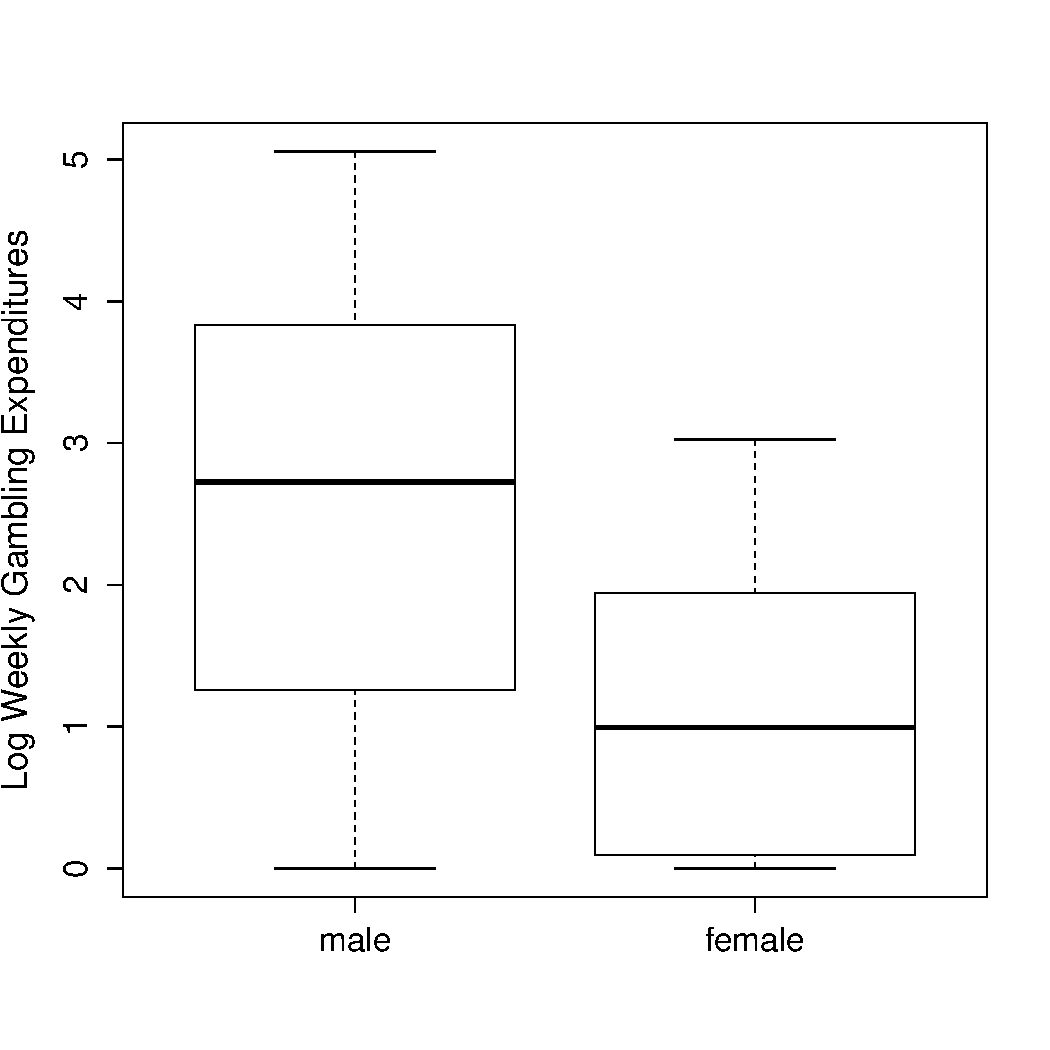
\includegraphics[width=.45\textwidth]{log_expend.pdf}
  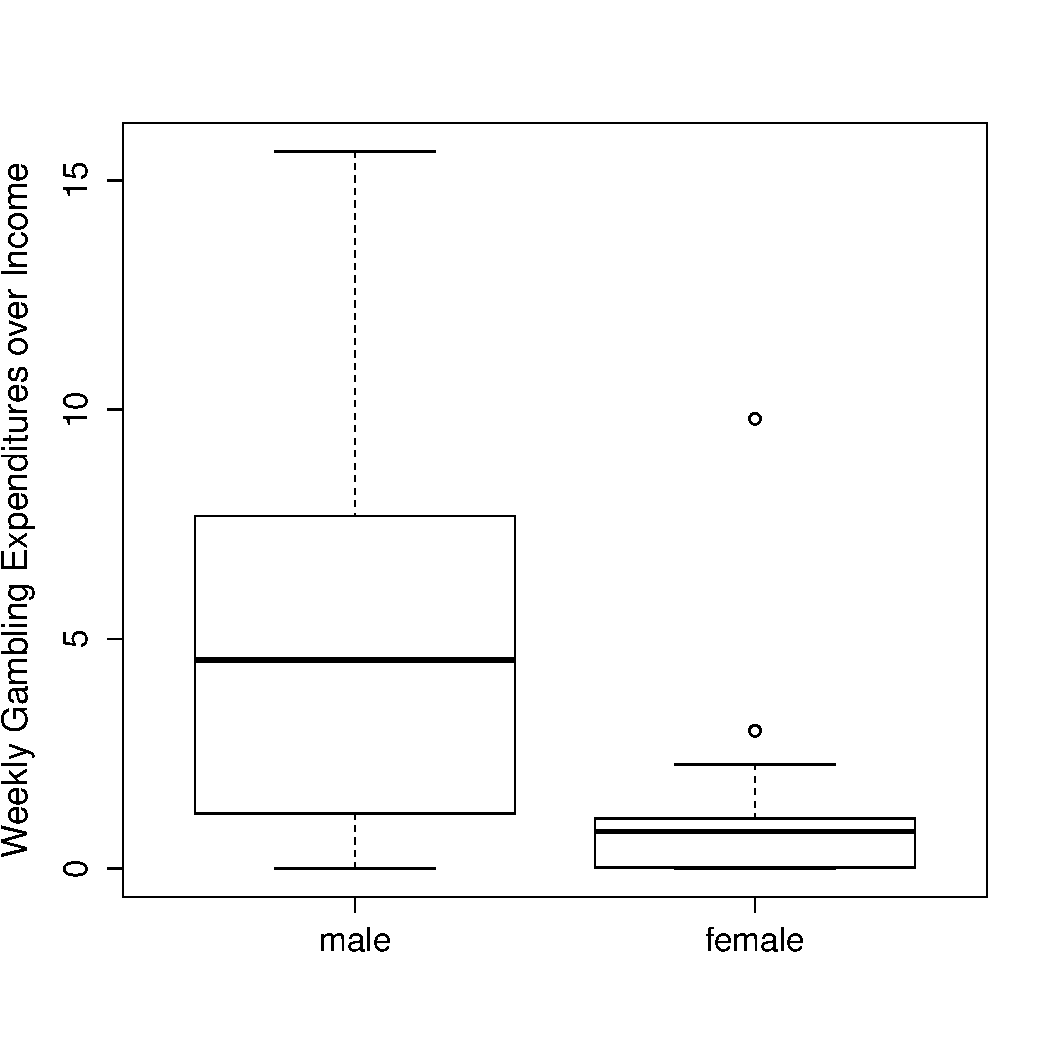
\includegraphics[width=.45\textwidth]{log_proportion.pdf}
  \end{solution}

  \problem{The dataset \texttt{prostate} is from a study on 97 men with prostate cancer who were due to receive a radical prostatectomy.  Make a numerical and graphical summary of the data as in question 6.}  
  
  \begin{solution}
    The data references the book \emph{Data} by Andrews and Herzber that was not conveniently available, so more
    detailed descriptions of the variables were not readily available.  Nine
    variables are briefly described in highly technical terms each quantitative
    except one.  We assume that the log cancer volume and log
    cancer weight are the response variables, with each of the remaining seven
    explanatory.  Presumably, the weight and volume of a cancerous tumor
    is difficult to predict without removing it, and the regime of diagnostics
    in this study are candidates for modeling the response.  
    
    Both the log cancer volume and log cancer weight are roughly bell shaped
    with the weight being slightly right skewed by a single outlier.  The
    assumption of normality in both of these responses may be appropriate. The
    ages of the patients range from 41 to 79 and are roughly bell shaped
    centered at 65 years old.  The ``log prostate specific antigen'' variable
    is also roughly bell shaped.  The variables ``log benign prostatic
    hyperplasia amount''(lbph), ``log capsular penetration''(lcp), and
    ``percentage Gleason scores 4 or 5''(pgg45) are each right skewed with lbph
    large amount of zero values.  A histogram of lbph without the zero values
    is bell-shaped.  The variable describing the ``Gleason score'' (gleason)
    has four possible values but was assumed to be quantitative since a
    positive correlation of the score value was observed with the log cancer
    volume. The binary categorical variable ``seminal vesical invasion'' (svi)  
    appeared to have higher volumes for where there was seminal vesical invasion
    than not. The weights were slightly higher of those with seminal vesical invasion
    but much less so.  Moreover, the variation in weights among those with 
    invasion was smaller than those without.  Also, noticeable distributional differences
    were observed in the side by side boxplots of in lcp pgg45 and lpsa among those with or without the invasion. 

    A matrix of scatter plots in the quantitative variables reveals a slight
    positive association between the cancer weight and volume.  If the outlying
    weight value is removed,  Pearson's correlation is $r=0.287$, otherwise
    $r=0.194$.  There is evidence for a positive correlation between age and
    both cancer volume and cancer weight ($r=0.225$ and $r=0.308$ respectively).  The lpsa
    variable has a very strong ($r=0.734$) positive relationship with the
    cancer volume and appears to be linear.  There is also a positive association with 
    weight, but less so.  The lbph variable has a positive association with weight ($r=0.435$), but
    appears to be non-linear with higher values resulting in higher weights. No other
    pronounced associations were observed, moreover, there did not appear to be any
    clear correlations between the explanatory quantitative variables.  

    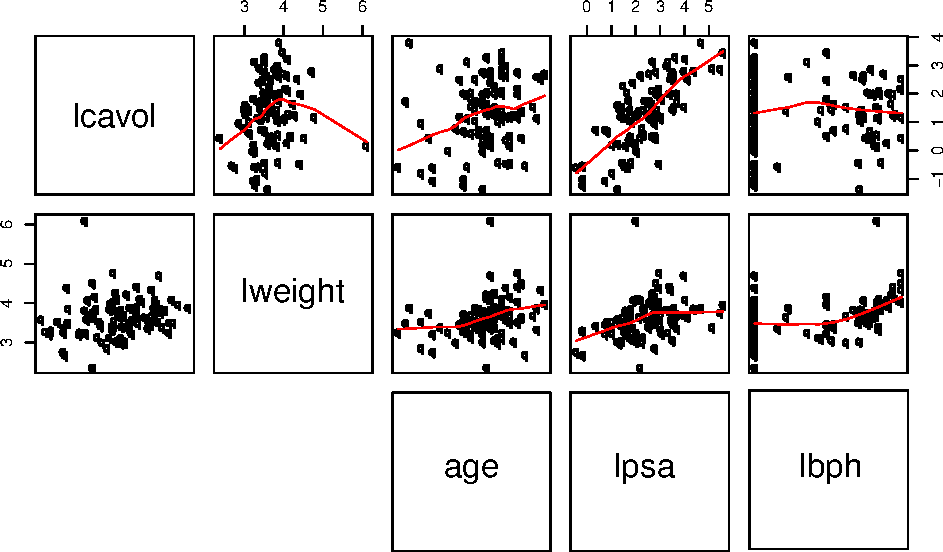
\includegraphics[width=.8\textwidth]{prostate_pairs.pdf}

  \end{solution}
\newpage
\begin{longproblem}
  Let $X$ be a random variable which follows a $t$-distribution with $k$ degrees of freedom.  

  \subproblem{ Show that $X^2$ has an $F$-distribution with 1 numerator and $k$ denominator degrees of freedom. }
  \begin{solution}
  We consider the transformations $g(x) = x^2$ which is one-to-one on $(-\infty,0)$ and $(0,\infty)$.  The relevant Jacobian is
  $|\frac 1{2\sqrt y}|.$ By transformation, the density of $X^2$ is
  \begin{align*}
    f_{X^2}(y) &= \frac 1{2 \sqrt y} \Big(f_X( -\sqrt y) I_{(-\infty,0)}(-\sqrt y) + f_X( \sqrt y ) I_{(0,\infty)}(\sqrt y)\Big)\\
    &= \frac1{\sqrt y}\cdot \frac{\Gamma\left(\frac{k+1}2\right)}{\sqrt{k\pi} \Gamma(k/2)}\left(1 + \frac{y}k\right)^{-(k+1)/2} I_{(0,\infty)}(y)\\
    &= y^{-1/2}\frac{\Gamma\left(\frac{k+1}2\right)}{\sqrt{k\pi} \Gamma(k/2)}\left(\frac k{k + y}\right)^{(k+1)/2} I_{(0,\infty)}(y)\\
    &= y^{-1/2}\frac{\Gamma\left(\frac{1+k}2\right)1^{1/2}k^{k/2}}{\Gamma(1/2) \Gamma(k/2)}\left(\frac {1}{k + y}\right)^{(k+1)/2} I_{(0,\infty)}(y)\\
    &= \frac{\Gamma\left(\frac{1+k}2\right)1^{1/2}k^{k/2}}{\Gamma(1/2) \Gamma(k/2)}\frac {y^{-1/2}}{(k + y)^{(k+1)/2}} I_{(0,\infty)}(y).\\
  \end{align*}
  This is the density for the desired $F$-distribution.
  \end{solution}
\end{longproblem}

  \subproblem{ Let $f_X(x|k)$ denote the probability density function (pdf) of $X$ as defined in part (a).  Show that:
  $$
    \lim_{k\to\infty} f_X(x|k) = \frac 1{\sqrt{2\pi}} \exp\{-x^2/2\},
  $$
  at each value of $x$ for $-\infty<x<\infty$.  Hence, argue that as $k\to \infty$, $X$ converges in distribution to a $N(0,1)$ random variable.}

  {\bf Solution:}

  The density for $T|k$ is given by 
    \begin{align*} 
    f_X(x|k) &= \frac{\Gamma\left(\frac{k+1}2\right)}{\sqrt{k\pi} \Gamma(k/2)}\left(1 + \frac{x^2}k\right)^{-(k+1)/2} \\
             &= \frac{\Gamma\left(\frac{k+1}2\right)}{\sqrt{k\pi} \Gamma(k/2)} \cdot \left(1 - \frac{-x^2/2}{k/2}\right)^{-k/2}\left(1 + \frac{x^2/2}{k/2}\right)^{1/2}. \\
  \end{align*}
  Note that as $k\to \infty$ the right factor
  $$
  \left(1 - \frac{-x^2/2}{k/2}\right)^{-k/2}\left(1 + \frac{x^2/2}{k/2}\right)^{1/2} \longrightarrow e^{-x^2/2} \cdot 1
  $$
  by the familiar formula $(1+x/n)^{-n} \to e^x$ and $1 + \frac{x^2/2}{k/2} \to 1$ for each fixed $x$.  
  
  Recall the identity $\Gamma(x + \alpha)/\Gamma(x) \stackrel{\dagger}\approx x^\alpha$ for large $x$.  Hence, as $k\to\infty$, the left factor is
  \begin{align*}
    \frac{\Gamma\left(\frac{k+1}2\right)}{\sqrt{k\pi} \Gamma(k/2)} &\approx \frac1{\sqrt{k\pi}} \left(\frac k2\right)^{1/2}\\
    &=\frac 1{\sqrt{2\pi}}.
  \end{align*}
  Since both factors are converging sequences, we have that the product of these limits is the desired quantity on the right hand side. 

  Note that each $f_X(x|k)$ is bounded above by $1$, hence Lebesgue's dominated convergence theorem allows for the passage of the limit in the CDF. I.e.
  \begin{align*}
  \lim_{k\to \infty} F_X(x|k) 
  &= \lim_{k\to \infty} \int_{-\infty}^x f_X(t|k)dt \\
  &= \int_{-\infty}^x \lim_{k\to \infty} f_X(t|k)dt \\
  &= \Phi(x)
  \end{align*}
  by the previous result.  Hence $X$ converges in distribution to $Z\sim N(0,1)$ as $k \to \infty$.
  
  %  we use Stirlings formula $ \Gamma(z+1) \approx \sqrt{2\pi z}\left(\frac ze\right)^z$ so the left factor is approximately
%  \begin{align*}
%    \frac 1{k\pi} \cdot \frac{\sqrt{2\pi \left(\frac{k-1}{2}\right) \left( \frac{k-1}{2e} \right)^ }}{\sqrt{2\pi \left(\frac{k-2}{2}\right) }}
%  \end{align*}

  The approximation in $^\dagger$ can be shown using Stirling's approximation for the gamma function.  Formally, this approximation means
  $$
    \lim_{x\to \infty} \frac{\Gamma(x + \alpha)/\Gamma(x)}{x^\alpha} = 1.
  $$
  Stirling says that 
  $$
    \log \Gamma(x) = \left(x-\frac 12\right)\log x - x + \frac 12 \log (2\pi) + O\left(\frac 1x\right),
  $$
  so
  \begin{align}
  \log\left( \frac{\Gamma(x + \alpha)/\Gamma(x)}{x^\alpha} \right) &=
  \left[ \left(x + \alpha -\frac 12\right)\log x - (x+\alpha) + \frac 12 \log (2\pi) + O\left(\frac 1x\right)\right] + \dots \nonumber\\
  & \quad\quad\quad\quad \dots-\left[ \left(x-\frac 12\right)\log x - x + \frac 12 \log (2\pi) + O\left(\frac 1x\right)\right] - \alpha \log x\nonumber\\
  &= \left(x +\alpha - \frac 12\right)\log\left(\frac{x+\alpha}x\right) - \alpha + O\left(\frac 1x\right).\label{series}
  \end{align}
  Note that $\ds{ \lim_{n\to\infty} \log\left(\frac{x+\alpha}x\right) = 0}$ and
  $$
  \lim_{x\to\infty}x\log\left(\frac{x + \alpha}x\right) =
  \lim_{x\to\infty}\frac{\ds{\frac{x}{x+\alpha}} \cdot \left( -\alpha x^{-2} \right)}{ -x^{-2} } =
  \alpha.
  $$
  Using these facts, and taking the limit as $x\to\infty$ in \eqref{series}, we have that the $\log$ of the ratio approaches $0$, and by continuity of $\log$, the limit of the ratio approaches 1.\qed
\end{document} 

